\section {Introduction to the analysis}

In this note, we present initial results of the tracker DAQ commissioning.
\section{Description of teststand setup}
  The tracker teststand, called TS1, includes one DRAC card and one DTC connected to the DAQ computer, 96 channels in total.
The ROC can be operated in two different data readout modes. In the first one the ROC emulates data itself without reading FPGAs. In the second mode the ROC reads digi FPGA.
 Most of the data were taken operating in the mode two with digi FPGAs, pulsed by their internal pulser.
  The pulser has two different frequencies,  31.29 MHz/(2$^7$+1), or approximately 250 kHz, 
and 31.29 MHz/(2$^9$+1), or approximately 60 kHz.
Event window is the time interval between two heartbeats (HB's). 
The logic of data taking is shown in Fig. \ref{fig:3}.
Pulses are represented with gray triangles and 
they are separated by the inverse of the generator frequency. We call $T_{gen}=1/f_{gen}$.
The event window, with the width of $T_{EW}$, that represents the distance between the proton pulses, 
was varied from 700 ns to 50 $\mu$s. 
The ROC firmware has an internal hit buffer which stores up to 255 hits.
That should be sufficient for the data taking.
Depending on $T_{gen}$ and $T_{EW}$, the data taking can proceed in two different modes:
  \begin{itemize}
  \item
    The event window is large enough , so the total number of generated hits is greater than 255. In this case
    the ROC hit buffer always gets filled up, and only the first 255 hits are read out;
  \item
    The total number of hits within the event window is less than 255.
    In this case the ROC hit buffer doesn't get filled up and the total number of hits can vary from one event to another.
  \end{itemize}
Each FPGA has its own pulse generator and pulse sequences from different generators are offset with respect to each other by a fixed $\Delta t$, fixed for the specific FPGA.
This offset can be a random number between 0 and $T_{gen}$.
Timing of generator pulses are uncorrelated with the beginning of the time window. Different number of hits can fit in the event window, as we can see in Fig.\ref{fig:3}.
Within one FPGA, pulses digitize in different channels and they have different timing, so they are offset of the order of nanoseconds.
Readout sequence is defined. All channels are readout in a specific sequence that doesn't change in different events. The sequence is shown in App.\ref{order}.

\begin{figure}[!h]
\centering
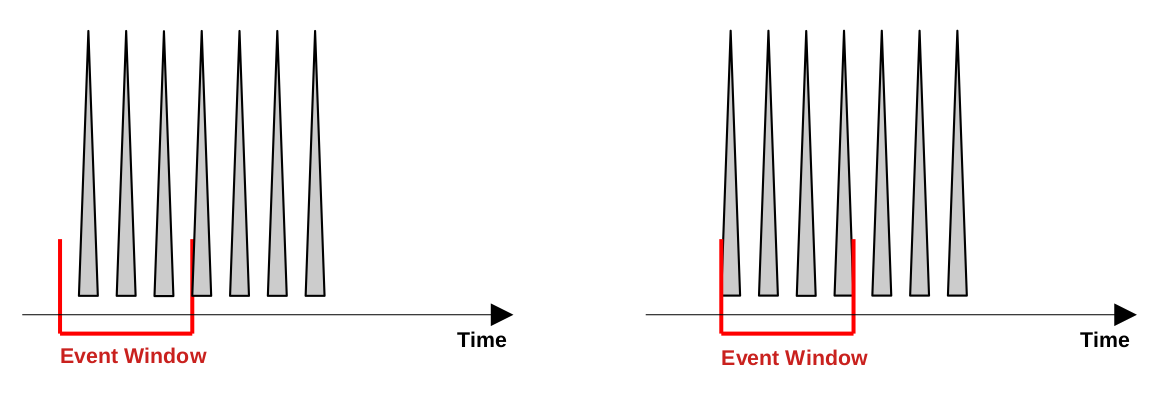
\includegraphics[width =0.8\textwidth]{figures/pdf/finalimg}
\caption{Graphic illustration of pulses in an event window.}
\label{fig:3}
\end{figure}
\section{Monte Carlo simulation}\label{MonteCarlo}
 
The ROC readout logic is purely digital, so the readout process can be simulated. 
The logic of the simulation is as follows.
The simulated parameters for each event are the number of hits in each channel and the total number of readout hits.
In the following sections, we call $occupancy$ the total number of hits versus channel number.

Given that the maximum allowable number of hits per event is 255, the simulation follows these steps:
\begin{itemize}
\item The event window starts at $t=0$s;
  \item The timing of the first pulse is generated randomly from 0 to $T_{gen}$, by sampling a uniform distribution;
    \item The previous pulses are generated subtracting from the first one a step of $T_{gen}$, until the absolute time of the pulse is greater than $T_{EW}$;
\item In each channel, pulses are generated in each channel following the readout sequence;
  \item After pulse generation, the readout continues until the count of hits reaches the maximum threshold of 255. 
\end{itemize}

The simulation takes into accounts the FPGAs offsets and the individual channel to channel offsets. 
We compared the simulated parameters with the measured ones. 

%%% Local Variables:
%%% mode: latex
%%% TeX-master: t
%%% End:

